\documentclass{article}

\usepackage{parskip}
\usepackage{microtype}
\usepackage{graphicx}
\usepackage{float}
\usepackage[colorlinks]{hyperref}
\usepackage[margin=2cm]{geometry}
\usepackage{helvet}
\usepackage{booktabs}
\usepackage[title]{appendix}
\usepackage{url}
\renewcommand{\familydefault}{\sfdefault}

\begin{document}
\section{Implementation}
Inside the main while loop,
the 2 inner for loop are parallelized by adding a \texttt{\#pragma acc parallel loop} just before the for declaration.
For the second while loop, a \texttt{reduction(max:worst\_dt)} is added to the pragma.
This allows the maximum dt to be calculated efficiently without any data races.

Variables \texttt{temp} and \texttt{temp\_prev} are rarely accessed by the host.
Repeated copying of them to and fro host and device is avoided by wrapping main while loop with a
\texttt{\#pragma acc data create(temp\_prev) create(temp)} block.
The \texttt{initialize} function is modified to perform initialization of \texttt{temp\_prev} on the device by addding
\texttt{\#pragma acc parallel loop present(temp\_prev)} before each for loop.
The initialize function is then moved inside the data block before the main while loop.

The only host code that accesses \texttt{temp} is \texttt{track\_progress} which is only called every 100 iterations.
It also only accesses \texttt{temp[HEIGHT]}.
\texttt{temp[HEIGHT]} is copied to the device every 100 iterations by adding a
\texttt{\#pragma acc update host(temp[HEIGHT])} just before \texttt{track\_progress(itr)}.

\section{Performance}
\begin{table}[H]
\centering
\begin{tabular}{@{}lrr@{}}
\toprule
exe             & mean time (ms) & stddev time \\ \midrule
laplace-acc-gpu & 133.54         & 0.17        \\
laplace-acc     & 459.45         & 1.83        \\
laplace-acc-opt & 128.20         & 0.48        \\
laplace-seq     & 2124.71        & 25.91       \\ \bottomrule
\end{tabular}
\caption{Comparison of different implementations on a xgpi node, h100-96 constraint. Each exe tested 10 times.}
\label{tab:tab-1}
\end{table}

As shown in table \ref{tab:tab-1},
my implementation (\path{laplace-acc-gpu}) achieves better performance than the provided \path{laplace-acc}. 

Performance was almost measured against variation in width and height.
Results are shown below in figure \ref{fig:graph}

\begin{figure}[H]
  \begin{center}
    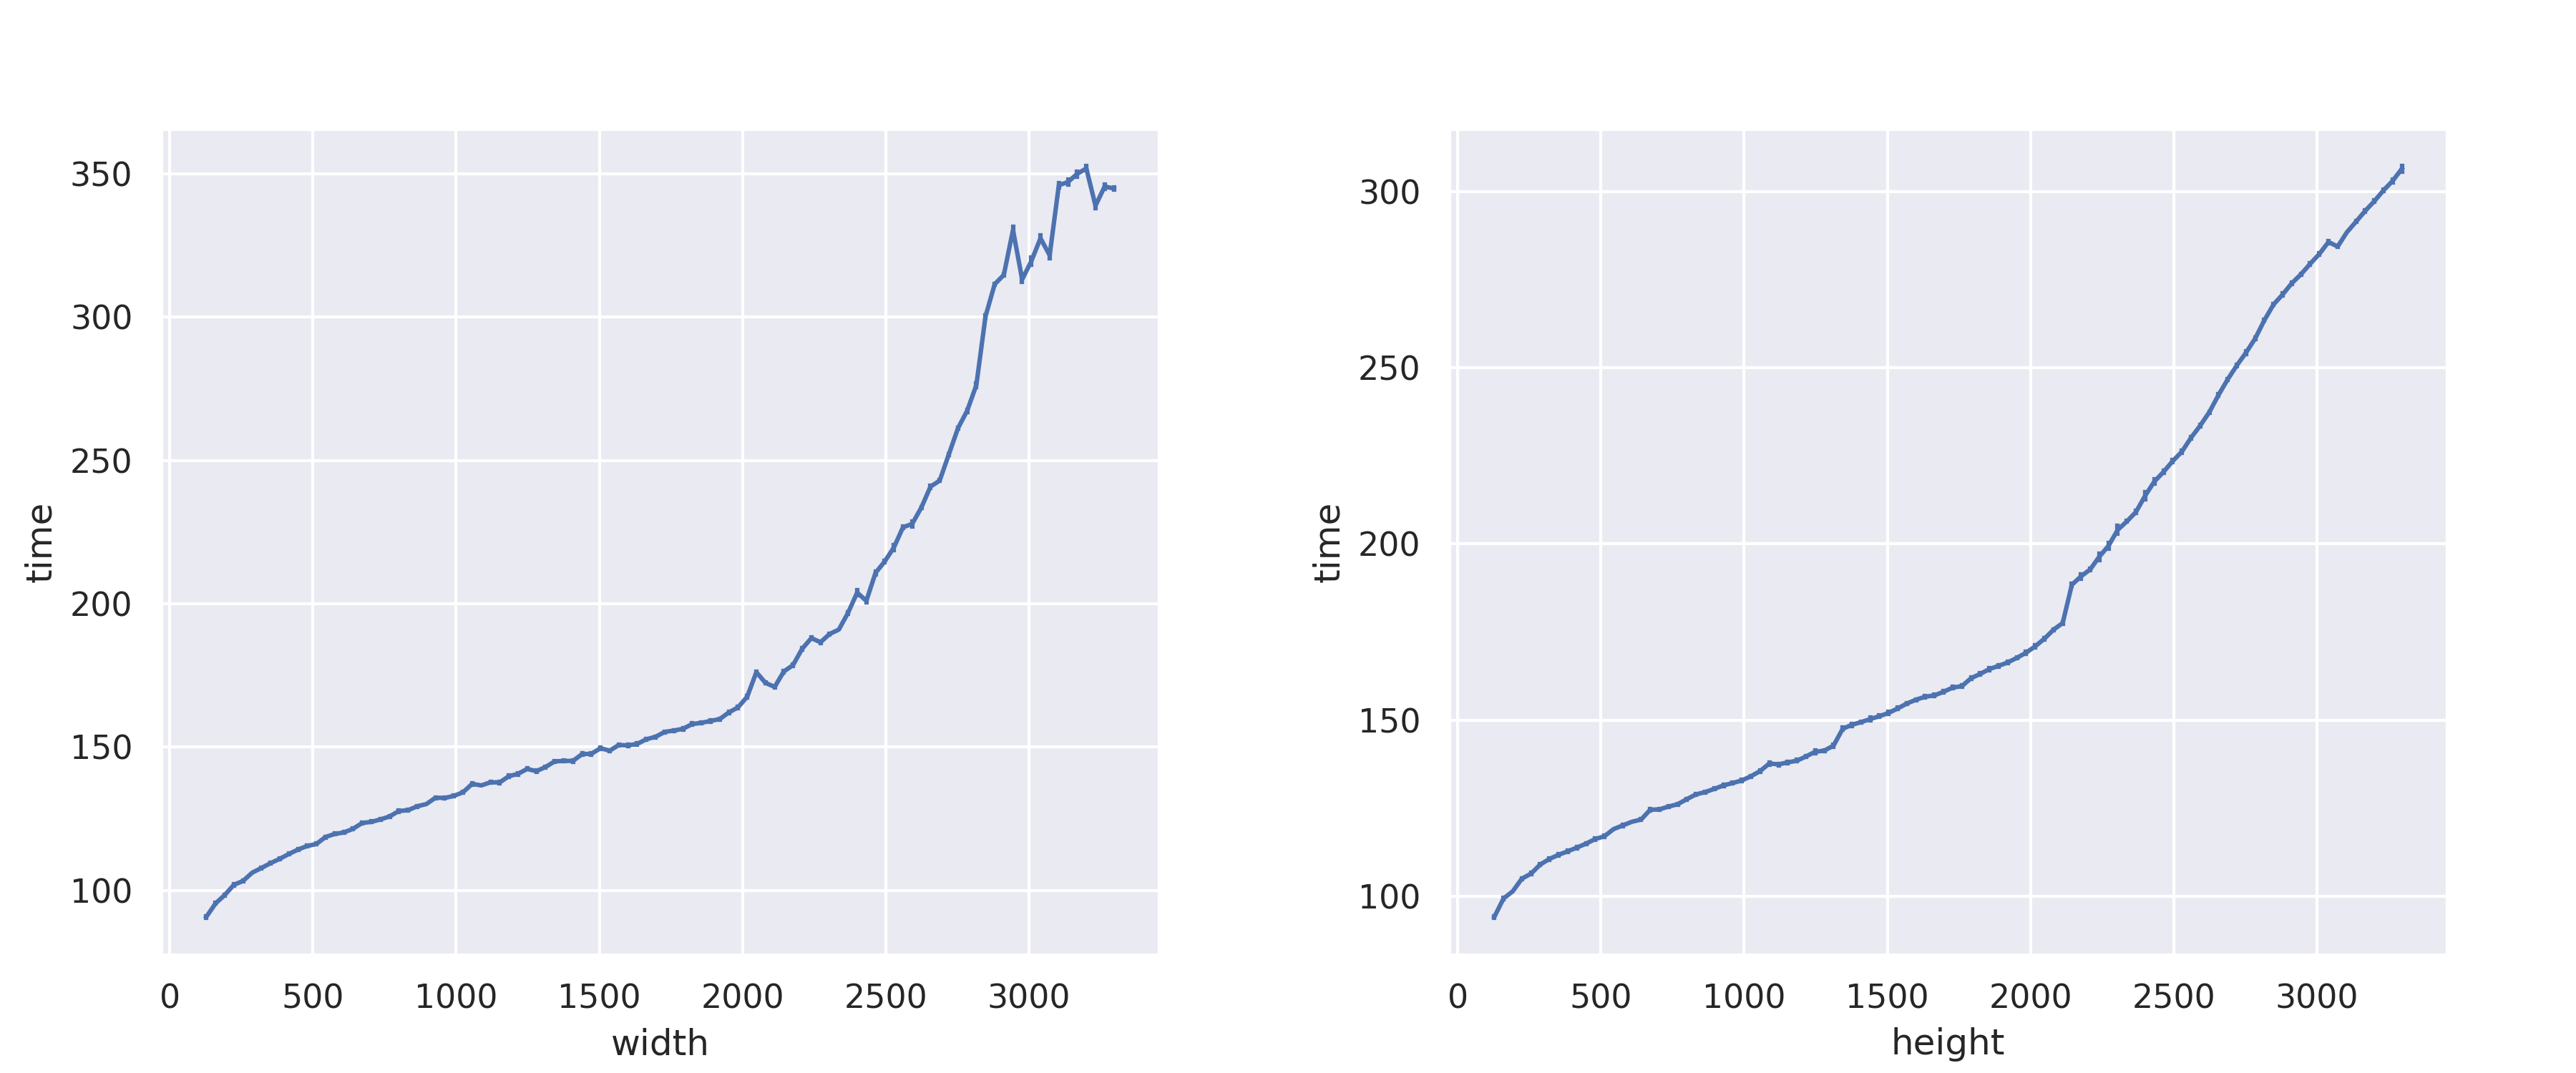
\includegraphics[width=0.95\textwidth]{figures/graph.png}
  \end{center}
  \caption{Time (ms) vs. Width / Height (error bars too small to see)}
  \label{fig:graph}
\end{figure}

As expected, runtime increases as width / height increases.
\clearpage

\begin{appendices}
  \section{Code}
  \begin{verbatim}
#include <stdlib.h>
#include <stdio.h>
#include <math.h>
#include "timer.hpp"

#define WIDTH      1024
#define HEIGHT     1024
#define TEMP_TOLERANCE 0.01

double temp[HEIGHT+2][WIDTH+2];
double temp_prev[HEIGHT+2][WIDTH+2];

void initialize();

void track_progress(int iter);

int main(int argc, char *argv[]) {
    int itr = 0;
    double worst_dt = 100;
    long long start, stop;


    #pragma acc data create(temp_prev) create(temp)
    {

    initialize();
    start = wall_clock_time();
    while ( worst_dt > TEMP_TOLERANCE ) {

        #pragma acc parallel loop
        for(int i = 1; i <= HEIGHT; i++) {
            for(int j = 1; j <= WIDTH; j++) {
                temp[i][j] = 0.25 * (temp_prev[i+1][j]
                        + temp_prev[i-1][j]
                        + temp_prev[i][j+1]
                        + temp_prev[i][j-1]);
            }
        }

        worst_dt = 0.0;

        #pragma acc parallel loop reduction(max:worst_dt)
        for(int i = 1; i <= HEIGHT; i++){
            for(int j = 1; j <= WIDTH; j++){
                double dt = fabs(temp[i][j] - temp_prev[i][j]);
                temp_prev[i][j] = temp[i][j];
                worst_dt = fmax(dt, worst_dt);
            }
        }

        if((itr % 100) == 0) {
            #pragma acc update host(temp[HEIGHT])
            track_progress(itr);
        }

        itr++;
    }
    }
    
    stop = wall_clock_time();

    printf("\nMax error at iteration %d was %f\n", itr-1, worst_dt);
    printf("Total time was %1.6f ms.\n", (float)(stop - start) / 1000000);
}

void initialize(){
    #pragma acc parallel loop present(temp_prev)
    for(int i = 0; i <= HEIGHT+1; i++){
        for (int j = 0; j <= WIDTH+1; j++){
            temp_prev[i][j] = 0.0;
        }
    }
    #pragma acc parallel loop present(temp_prev)
    for(int i = 0; i <= HEIGHT+1; i++) {
        temp_prev[i][0] = 0.0;
        temp_prev[i][WIDTH+1] = (100.0/HEIGHT)*i;
    }
    #pragma acc parallel loop present(temp_prev)
    for(int j = 0; j <= WIDTH+1; j++) {
        temp_prev[0][j] = 0.0;
        temp_prev[HEIGHT+1][j] = (100.0/WIDTH)*j;
    }
}
void track_progress(int itr) {
    printf("---------- Iteration number: %d ------------\n",
            itr);
    for(int i = 0; i <= HEIGHT; i += (HEIGHT/8)) {
        printf("[%d,%d]: %5.2f  ", i, HEIGHT, temp[HEIGHT][i]);
    }
    printf("\n");
}
  \end{verbatim}

  \clearpage
  \section{Test Scripts}
  Compilation, running, benchmarking, and parsing results were performed with the following
  \href{https://www.nushell.sh/}{nushell} scripts

  \subsection{Benchmark script}
  \begin{verbatim}
let my_exe = "laplace-acc-gpu"
let binaries = [$my_exe, "laplace-acc",  "laplace-acc-opt", "laplace-seq"]

^nvc++ -acc=gpu -Minfo=acc -fast  -o $my_exe ./laplace-acc.cpp | ignore

$binaries | each {
  let exe = $in
  1..10 | each {
    let out = ^$'./($exe)' | complete | update stdout {lines} | update stderr {lines}
    let time = $out.stdout | parse -r 'Total time was (?<time>[.\d]+) ms' | 
      get -i 0.time |
      default nan |
      into float
    {exe: $exe, time: $time} | to json -r | print
  }
} | ignore
  \end{verbatim}
  
  \subsection{Measurement script}
\begin{verbatim}
def generate_tests [] {
  let height_range = 128..160.. | take 100
  let width_range = 128..160.. | take 100
  
  let height_test = $height_range | par-each {
    {height: $in, width: 1024, test: height}
  }
  let width_test = $width_range | par-each {
    {height: 1024, width: $in, test: width}
  }
  $height_test | append $width_test
}

def run_test [] {
  let config = $in
  let tmp_dir = mktemp -d
  let exe = $tmp_dir | path join exe
  let compile_result = nvc++ -acc=gpu -Minfo=acc -fast -DHEIGHT=($config.height) -DWIDTH=($config.width) -o $exe ./laplace-acc.cpp | complete | update stdout {lines} | update stderr {lines}
  
  if $compile_result.exit_code != 0 {
    rm $tmp_dir
    return $config | insert compile $compile_result
  }

  let runs = 1..5 | each {
    let output = ^($exe) | complete | update stdout {lines} | update stderr {lines}
    let time = $output.stdout | parse -r 'Total time was (?<time>[.\d]+) ms' |
      get -i 0.time |
      default NaN |
      into float

    $output | insert time $time
  }

  $config | insert compile $compile_result | insert runs $runs | to json -r | print

  rm -r $tmp_dir
}

def main [] {
  generate_tests | each {run_test} | ignore
}
\end{verbatim}
\section{Raw Data}
Raw data obtained from test scripts above can be found in
\url{https://github.com/ginloy/CS3210-Labs/blob/main/L6/laplace-test-out.jsonl} and
\url{https://github.com/ginloy/CS3210-Labs/blob/main/L6/bench-out.jsonl}.

Data analysis and graphs were done using python, polars, matplotlib, and seaborn in
\url{https://github.com/ginloy/CS3210-Labs/blob/main/L6/graphs.ipynb}
\end{appendices}

\end{document}
